\documentclass[border=2pt]{standalone}
\usepackage{tikz}
\usetikzlibrary{arrows.meta,positioning,calc,fit,backgrounds,shapes.geometric}
\usepackage{amsmath,amssymb}
\usepackage{times}
\definecolor{ink}{HTML}{243447}
\definecolor{cA}{HTML}{4477AA}
\definecolor{cB}{HTML}{CC6677}
\definecolor{cAu}{HTML}{44AA99}
\definecolor{cS}{HTML}{CCAA33}
\definecolor{grn}{HTML}{228833}
\definecolor{rose}{HTML}{AA3377}
\definecolor{inst}{HTML}{F2E3B3}
\tikzset{
 pap/.style={circle,draw=ink,line width=.6pt,minimum size=15pt,inner sep=0pt,font=\scriptsize\bfseries,text=white},
 aut/.style={rectangle,draw=ink,line width=.6pt,minimum size=13pt,inner sep=0pt,fill=cAu,font=\scriptsize\bfseries,text=white},
 sub/.style={diamond,draw=ink,line width=.6pt,minimum size=17pt,inner sep=0pt,fill=cS,font=\scriptsize\bfseries,text=white},
 gone/.style={draw=ink!35,fill=ink!8,text=ink!40,dashed},
 ed/.style={draw=ink,line width=.7pt},
 msg/.style={-{Stealth[length=4pt]},line width=.9pt,draw=rose},
 ptitle/.style={font=\footnotesize\bfseries,text=ink,anchor=west},
 note/.style={font=\scriptsize,text=ink,align=center},
}

\tikzset{
 stage/.style={draw=ink!50,rounded corners=3pt,line width=.5pt,minimum width=2.78cm,minimum height=3.3cm,anchor=north west},
 stnum/.style={circle,fill=ink,text=white,font=\scriptsize\bfseries,inner sep=1.2pt},
 sname/.style={font=\scriptsize\bfseries,text=ink,anchor=west},
 small/.style={font=\fontsize{5.9}{6.8}\selectfont,text=ink,align=center},
 vec/.style={draw=ink,fill=#1,minimum width=4pt,minimum height=11pt,inner sep=0pt},
 flow/.style={-{Stealth[length=4pt]},line width=1pt,draw=ink!60},
 est/.style={rectangle,draw=grn,fill=grn!15,line width=.5pt,minimum size=6pt,inner sep=0pt},
 fst/.style={circle,fill=rose,inner sep=1.6pt},
}
\begin{document}
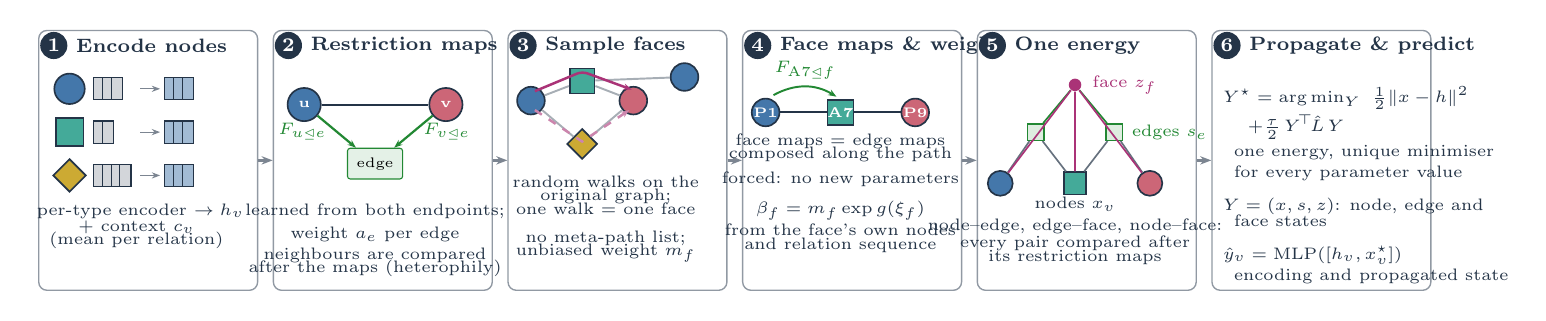
\begin{tikzpicture}
\def\W{2.98}
\foreach \i/\t in {0/Encode nodes,1/Restriction maps,2/Sample faces,3/Face maps \& weight,4/One energy,5/Propagate \& predict}{
  \node[stage] (B\i) at (\i*\W,0) {};
  \node[stnum] at ($(B\i.north west)+(0.2,-0.2)$) {\the\numexpr\i+1\relax};
  \node[sname] at ($(B\i.north west)+(0.36,-0.2)$) {\t};
}
\foreach \i in {0,...,4}{ \pgfmathtruncatemacro\j{\i+1} \draw[flow] (B\i.east)--(B\j.west); }
% ---- 1 encode
\begin{scope}[shift={(0.25,-0.75)}]
 \node[pap,fill=cA,minimum size=11pt] at (0.15,0) {};
 \node[aut,minimum size=10pt] at (0.15,-0.55) {};
 \node[sub,minimum size=12pt] at (0.15,-1.1) {};
 \foreach \y/\w in {0/3,-0.55/2,-1.1/4}{\foreach \k in {1,...,\w}{\node[vec=ink!20,minimum height=8pt] at (0.42+\k*0.11,\y) {};}}
 \foreach \y in {0,-0.55,-1.1}{\draw[-{Stealth[length=3pt]},ink!60] (1.05,\y)--(1.3,\y);
   \foreach \k in {1,...,3}{\node[vec=cA!50,minimum height=8pt] at (1.32+\k*0.11,\y) {};}}
 \node[small] at (1.05,-1.55) {per-type encoder $\to h_v$};
 \node[small] at (1.0,-1.85) {+ context $c_v$\\[-2pt](mean per relation)};
\end{scope}
% ---- 2 restriction maps
\begin{scope}[shift={(\W+0.25,-0.95)}]
 \node[pap,fill=cA,minimum size=12pt] (u) at (0.15,0) {\tiny u};
 \node[pap,fill=cB,minimum size=12pt] (v) at (1.95,0) {\tiny v};
 \node[draw=grn,fill=grn!12,rounded corners=1pt,minimum width=0.5cm,minimum height=0.32cm,font=\tiny] (es) at (1.05,-0.75) {edge};
 \draw[ed] (u)--(v);
 \draw[-{Stealth[length=3pt]},grn,line width=.8pt] (u) -- node[small,left,text=grn]{$F_{u\trianglelefteq e}$} (es);
 \draw[-{Stealth[length=3pt]},grn,line width=.8pt] (v) -- node[small,right,text=grn]{$F_{v\trianglelefteq e}$} (es);
 \node[small] at (1.05,-1.35) {learned from both endpoints;};
 \node[small] at (1.05,-1.65) {weight $a_e$ per edge};
 \node[small] at (1.05,-2.0) {neighbours are compared\\[-2pt]after the maps (heterophily)};
\end{scope}
% ---- 3 WISP
\begin{scope}[shift={(2*\W+0.3,-0.9)}]
 \node[pap,fill=cA,minimum size=10pt] (s1) at (0,0) {};
 \node[aut,minimum size=9pt] (s2) at (0.65,0.25) {};
 \node[pap,fill=cB,minimum size=10pt] (s3) at (1.3,0) {};
 \node[sub,minimum size=11pt] (s4) at (0.65,-0.55) {};
 \node[pap,fill=cA,minimum size=10pt] (s5) at (1.95,0.3) {};
 \draw[ed,ink!40] (s1)--(s2)--(s3) (s1)--(s4)--(s3) (s2)--(s5);
 \draw[-{Stealth[length=3pt]},rose,line width=.9pt,rounded corners=2pt] ($(s1)+(0.05,0.12)$)--($(s2)+(0,0.12)$)--($(s3)+(-0.02,0.14)$);
 \draw[-{Stealth[length=3pt]},rose!60,line width=.9pt,dashed] ($(s1)+(0.05,-0.12)$)--($(s4)+(0,0.03)$)--($(s3)+(-0.05,-0.12)$);
 \node[small] at (0.95,-1.2) {random walks on the\\[-2pt]original graph;\\[-2pt]one walk = one face};
 \node[small] at (0.95,-1.85) {no meta-path list;\\[-2pt]unbiased weight $m_f$};
\end{scope}
% ---- 4 face maps + weight
\begin{scope}[shift={(3*\W+0.3,-1.05)}]
 \node[pap,fill=cA,minimum size=10pt] (q1) at (0,0) {\tiny P1};
 \node[aut,minimum size=9pt] (q2) at (0.95,0) {\tiny A7};
 \node[pap,fill=cB,minimum size=10pt] (q3) at (1.9,0) {\tiny P9};
 \draw[ed] (q1)--(q2)--(q3);
 \draw[-{Stealth[length=3pt]},grn,line width=.7pt] ($(q1)+(0.1,0.22)$) to[bend left=30] node[small,above=-1pt,text=grn]{$F_{\mathrm{A7}\trianglelefteq f}$} ($(q2)+(-0.05,0.2)$);
 \node[small] at (0.95,-0.45) {face maps = edge maps\\[-2pt]composed along the path};
 \node[small] at (0.95,-0.85) {forced: no new parameters};
 \node[small] at (0.95,-1.25) {$\beta_f = m_f\exp g(\xi_f)$};
 \node[small] at (0.95,-1.6) {from the face's own nodes\\[-2pt]and relation sequence};
\end{scope}
% ---- 5 energy on three levels
\begin{scope}[shift={(4*\W+0.3,-0.75)}]
 \node[fst] (z) at (0.95,0.05) {};
 \node[small,anchor=west,text=rose] at (1.05,0.05) {face $z_f$};
 \node[est] (e0) at (0.45,-0.55) {};
 \node[est] (e1) at (1.45,-0.55) {};
 \node[small,anchor=west,text=grn] at (1.55,-0.55) {edges $s_e$};
 \node[pap,fill=cA,minimum size=9pt] (n1) at (0,-1.2) {};
 \node[aut,minimum size=8pt] (n2) at (0.95,-1.2) {};
 \node[pap,fill=cB,minimum size=9pt] (n3) at (1.9,-1.2) {};
 \node[small] at (0.95,-1.47) {nodes $x_v$};
 \draw[grn,line width=.6pt] (z)--(e0) (z)--(e1);
 \draw[ink!70,line width=.6pt] (n1)--(e0) (n2)--(e0) (n2)--(e1) (n3)--(e1);
 \draw[rose,line width=.6pt] (z)--(n1) (z)--(n2) (z)--(n3);
 \node[small] at (0.95,-1.75) {node--edge, edge--face, node--face:};
 \node[small] at (0.95,-2.05) {every pair compared after\\[-2pt]its restriction maps};
\end{scope}
% ---- 6 propagate
\begin{scope}[shift={(5*\W+0.05,-0.75)}]
 \node[small,align=left,anchor=north west] at (-0.02,0.15) {$Y^\star=\arg\min_Y\ \tfrac12\|x-h\|^2$\\[1pt]\hspace*{1.2em}$+\tfrac\tau2\,Y^{\!\top}\!\hat L\,Y$\\[2pt]
 \phantom{x}one energy, unique minimiser\\[1pt]\phantom{x}for every parameter value\\[5pt]
 $Y=(x,s,z)$: node, edge and\\[-1pt]\phantom{x}face states\\[5pt]
 $\hat y_v=\mathrm{MLP}([h_v,x^\star_v])$\\[1pt]\phantom{x}encoding and propagated state};
\end{scope}
\end{tikzpicture}
\end{document}
